  \let\negmedspace\undefined
\let\negthickspace\undefined
\documentclass[journal]{IEEEtran}
\usepackage[a5paper, margin=10mm, onecolumn]{geometry}
\usepackage{lmodern} % Ensure lmodern is loaded for pdflatex
\usepackage{tfrupee} % Include tfrupee package

\setlength{\headheight}{1cm} % Set the height of the header box
\setlength{\headsep}{0mm}     % Set the distance between the header box and the top of the text

\usepackage{gvv-book}
\usepackage{gvv}
\usepackage{cite}
\usepackage{amsmath,amssymb,amsfonts,amsthm}
\usepackage{algorithmic}
\usepackage{graphicx}
\usepackage{textcomp}
\usepackage{xcolor}
\usepackage{txfonts}
\usepackage{listings}
\usepackage{enumitem}
\usepackage{mathtools}
\usepackage{gensymb}
\usepackage{comment}
\usepackage[breaklinks=true]{hyperref}
\usepackage{tkz-euclide} 
\usepackage{listings}                                      
\def\inputGnumericTable{}                                 
\usepackage[latin1]{inputenc}                                
\usepackage{color}                                            
\usepackage{array}                                            
\usepackage{longtable}
\usepackage{multicol}
\usepackage{calc}                                             
\usepackage{multirow}                                         
\usepackage{hhline}                                           
\usepackage{ifthen}                                           
\usepackage{lscape}
\begin{document}
	
	\bibliographystyle{IEEEtran}
	\vspace{3cm}
	
	\title{4.1.1.7}
	\author{EE24BTECH11059 - Y Siddhanth}
	% \maketitle
	% \newpage
	% \bigskip
	{\let\newpage\relax\maketitle}
	
	\renewcommand{\thefigure}{\theenumi}
	\renewcommand{\thetable}{\theenumi}
	\setlength{\intextsep}{10pt} % Space between text and floats
	
	
	\numberwithin{equation}{enumi}
	\numberwithin{figure}{enumi}
	\renewcommand{\thetable}{\theenumi}
	
	
\textbf{Question}:\\
Find the roots of the equation \( (x + 2)^3 = 2x (x^2 - 1) \)
\\
\textbf{Solution: }\\
First, we simplify the given equation,
\begin{align}
	x^3 -2x^2 - 6x - 8 = 0
\end{align}
We can solve the above equation using fixed point iterations. First we separate $x$, from the above equation and make an update equation of the below sort.
\begin{align}
	x = g\brak{x} \implies x_{n+1} = g\brak{x_n}
\end{align}
Applying the above update equation on our equation, we get
\begin{align}
	x_{n+1} = 	\frac{x_n^3 -2x_n^2 - 8}{6}
\end{align}
Now we take an initial value $x_0$ and iterate the above update equation. But we realize that the updated values always approach infinity for any initial value. \\
Thus we will alternatively use Newton's Method for solving equations.
\begin{align}
	x_{n+1} = x_n - \frac{f\brak{x_n}}{f^{\prime}\brak{x_n}} 
\end{align}
Where we define $f\brak{x}$ as, 
\begin{align}
	f\brak{x} = x^3 -2x^2 - 6x - 8 \\
	f^{\prime}\brak{x} = 3x^2 -4x - 6 
\end{align}
Thus, the new update equation is, 
\begin{align}
	x_{n+1} = x_n - \frac{x_n^3 -2x_n^2 - 6x_n - 8}{3x_n^2 -4x_n - 6 } 
\end{align}
Taking the initial guess as $x_0 = 1$, we can see that $x_n$ converges at the 43rd iteration with x as,
\begin{align}
	x = 4
\end{align}
Alternatively, we can use the Secant method for solving equations.
\begin{align}
	x_{n+1} = x_n + f\brak{x_n}\frac{x_{n} -  x_{n-1}}{f(x_{n}) -  f(x_{n-1})}
\end{align}
Newton's method is very powerful but has the disadvantage that the derivative may sometimes be a far more difficult expression than \(f(x)\) itself and its evaluation therefore it may be more computationally expensive. The secant's method is more computationally cheap as the equation of the derivative is avoided by taking 2 starting points.\\ 
Taking the initial guesses as $x_0 = 1, x_1 = 2$, we see that $x_n$ converges in 36 iterations with x as,
\begin{align}
	x = 4
\end{align} 
	\begin{figure}[h!]
		\centering
		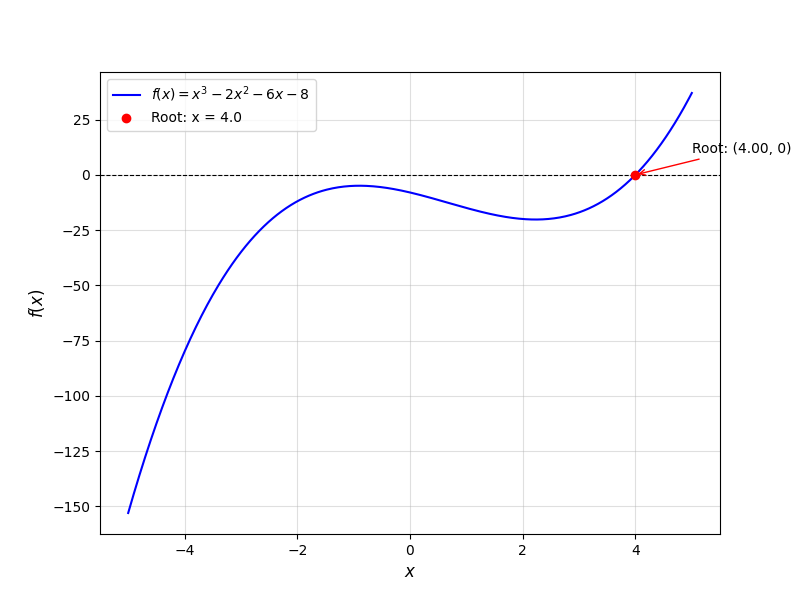
\includegraphics[width=\columnwidth]{figs/fig1.png}
		\caption{Solution of the given function}
		\label{stemplot}
	\end{figure}
	
\end{document}  